% Chapter 1

\chapter{Prototype I} % Main chapter title

\label{prototype1chapter} % For referencing the chapter elsewhere, use \ref{Chapter1} 

\lhead{Chapter \ref{prototype1chapter}. \emph{Prototype I}} % This is for the header on each page - perhaps a shortened title
%----------------------------------------------------------------------------------------
\section{Development of the Prototype}
The initial task that I conducted was to develop the first version of the application prototype. The prototype had features that allow monitoring of physical activity and diet of an individual. The manipulation of user interfaces of the app was specifically targeted to help-givers/intermediary users. I designed the prototype in such a way that it encourages one help-giver to work together with one help-seeker by forming one pair of users. In order to make the act of helping both important and meaningful to intermediary users, the first message displayed when opening the app was explicit: an intermediary user is helping someone they know (or care about) manage their wellness. In the case of motivating ongoing use, the app included gamification features, where each pair could be awarded points, badges, nice-looking gardens, and fish tanks. The essence of having these features was to enable pairs of users to have a set of challenges that would promote competence, one of the core aspects of self-determination theory. In addition to the aforementioned features, within each pair of users' garden and fish tank, there was a Facebook social plug-in that allowed members from different teams/pairs to comment on or like each other. The presence of these social features was to promote relatedness, which is another aspect of self-determination theory. The app also utilized Facebook groups to give feedback or remind users to engage with the application. The first prototype did not explicitly have any functionality to support autonomy. The information flow on the high-level representation of the system to encourage intermediated use was as depicted in Figure \ref{figure:prototype_1}. 

\begin{figure}[htbp]
  \centering
    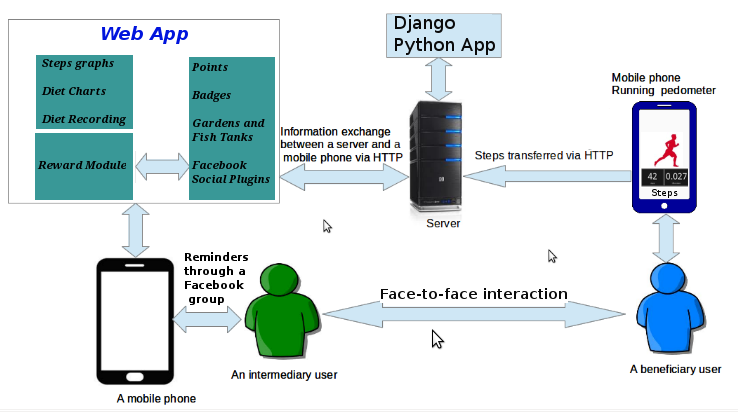
\includegraphics[width=0.8\textwidth]{Figures/prototype_1a.png}
    \rule{35em}{0.5pt}
  \caption{Information flow in the first prototype.}
  \label{figure:prototype_1}
\end{figure}

I developed a web app using a combination of several web technologies such as HTML, JQuery, JavaScript and CSS on the client side, while I achieved the implementation of the server side using Django Python framework. Sample screen-shots of the prototype are shown in Figure \ref{figure:prototype_1_screens}. 

\begin{figure}[htbp]
  \centering
    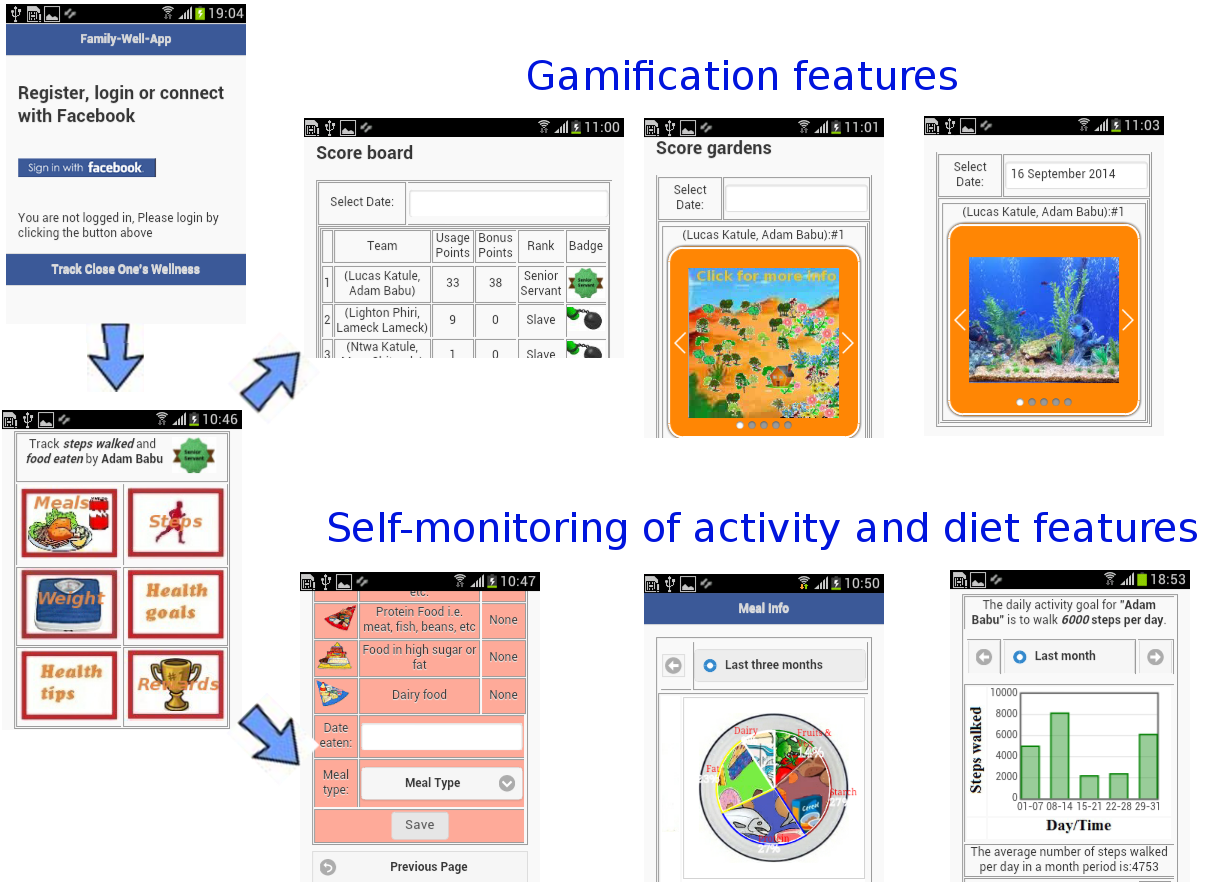
\includegraphics[width=0.8\textwidth]{Figures/Version1/Prototype1Screenshots.png}
    \rule{35em}{0.5pt}
  \caption{Sample screen-shots of the first prototype.}
  \label{figure:prototype_1_screens}
\end{figure}

The system could authenticate users through Facebook accounts of intermediary users. I developed the pedometer app (Figure \ref{figure:pedometer_screen}) in Android environment by extending the open source code downloaded from Github\footnote{https://github.com/bagilevi/android-pedometer}. 

\begin{figure}[htbp]
  \centering
    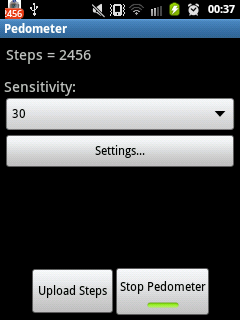
\includegraphics[width=0.3\textwidth]{Figures/pedometerapp.png}
    \rule{35em}{0.5pt}
  \caption{The native pedometer app.}
  \label{figure:pedometer_screen}
\end{figure}

The pedometer code allowed readings from the phone's accelerometer (built-in sensor to detect physical activity) that are above a certain threshold to be detected as bodily bounces from physical activity. The data was then stored in the SQLITE database on the phone. The pedometer app included the capability for transferring data to the server after every 30 minutes, but users could also press an upload button on the pedometer app for immediate transfer of footsteps to the server. The pedometer was not calibrated to differentiate varying intensity of physical activity as it was not an important aspect for this study. A single body bounce was treated as one step regardless of its intensity. 

This prototype aimed at encouraging an increase in physical activity and  a decrease of sedentary behaviours through informing individuals (help-seekers) of their current behaviour trends. In addition, individuals could monitor whether they were eating healthily or not. Some visualization techniques that are similar to this have previously been used  in systems that were designed for direct users such as Fish'n'Steps~\citep{lin2006:fish}, Ubifit~\citep{klasnja2009:using}  and the Few Touch application~\citep{arsand:mobile}. In the reported study in this chapter, the way the fish tank or garden appeared depended on how many footsteps had been captured.  

Another aspect of interface design, was the idea of using a plate to show distribution of meals' nutrition mimicked a practice that was used by dietitians at the hospital where we conducted the contextual enquiry reported on in the previous chapter. In this design metaphor, the amount of each food group that needs to be consumed is presented as a bisector of a pie chart. 
\section{Prototype Evaluation}
There was a slight change of plan  due to contention about the study design and ethical implications when dealing with patients as per requirements of the Faculty of Health Sciences Human Research Ethics Committee (FHS-HREC) of the University of Cape Town. FHS-HREC was interested in having clinical outcomes as one of the expected outputs. These requirements were going to increase the scope of the work, of which the main area of contribution was supposed to be in human-computer interaction. Also, the envisaged technology was only under research; hence it was not expected to be comprehensive enough and ready for any clinical trials even after completion of all evaluations that were meant to be carried out throughout this research. Therefore, I had to look for a different group of participants outside hospital settings. This involved reapplication for ethical approval to an institution body different from the first one that approved the study reported on in the previous chapter (Chapter \ref{contextualenqchapter}). This time the ethical approval was granted by the Faculty of Science Research Ethics Committee (FSREC) of the University of Cape Town (see Appendix B).

In order to evaluate the aforementioned prototype, I recruited participants through help from \textbf{\textit{Mamelani Projects}}\footnote{http://www.mamelani.org.za/}, an NGO
based in Cape Town. This NGO was conducting out outreach programmes on health education in less-privileged communities, and training women on issues of HIV/AIDS, nutrition and gender equality. 

The NGO helped to recruit participants among people who were part of their training in Philippi township. Criteria for recruitment were as follows: (1) participants that were mid-aged and above (contextual enquiry suggested that most prospective beneficiaries could be above mid-aged) and (2) participants who had an intermediary person willing to work with them (someone they trusted or close to them). The NGO identified the targeted participants that met the inclusion criteria. We recruited a total of six adult participants, all of them women above mid-age (\textgreater= 35 years of age). Each of the adults brought one intermediary to form a pair. Three intermediaries were girls between 19 and 23 years of age; the remaining three intermediaries were boys between 14 and 19 years of age. 

In the next step, I informed participants of their rights and that the study will collect their information. Both adults and their respective intermediaries signed consent forms, except those intermediaries who were minors; these signed assent forms that were approved by their parents/guardians. 

The next step entailed training the intermediaries to use the app. I deployed the application in the field from the end of October 2014 to the beginning of December 2014. In order to limit potential complications from deploying the intervention on multiple platforms, each pair of participants was given one Android phone (Samsung GT-S5300) running the pedometer app. I had set each pedometer with the identity of a pair in order to distinguish readings from different pairs. Participants were required to utilize the web application hosted at the University of Cape Town by using a web browser built into their phones. In order to retain participants in the study, each intermediary participant and each beneficiary participant who remained as part of the study received ZAR30 (USD3) worth of airtime every week for the duration of the study. I collected qualitative feedback in the middle and at the end of the study. All names used in the qualitative feedback are pseudonyms to protect the identity of the participants.
\section{Findings}
Observations and qualitative feedback from the six cases/pairs are presented below. The first three pairs were parents working with their children, while the remaining three pairs were an adult working with either a close or distant relative.
\subsection*{\textbf{Pair 1: Mother and Son}}
This pair was a 17-year-old called ``\textbf{Jabulani}'' and his mother ``\textbf{Nandipha}''. Jabulani lived with his mother and siblings. He appeared to be passionate about engaging with a cellphone. Below he describes the intimate relationship he has with his cellphone.

\userquote{\textbf{Jabulani}} {``There is a time I lost my cellphone. It was like the end of the world to me, because I didn't have anything to play with.''}

This shows that a cellphone could be a source of intrinsic motivation for young users in this context. 

He mentioned that he felt happy helping his mother. He also articulated the reason for helping his mother was that he felt it was his duty, since she had taken care of him when he was growing up. 

\userquote{\textbf{Jabulani}} {``I feel happy when I am helping her, because she helped me when I was growing up. So it is my turn to help her''}

\textbf{Nandipha} also felt very happy being helped by her son and said that she thinks her son is more brilliant than her with technology, and that she gets to know things because of him. 

Jabulani and Nandipha were the first to engage with the app for at least three different days. Then all of a sudden, they stopped using it. When I asked them what prevented them from using the app, they replied that, they were more conscious about airtime and so did not log in more often. There were times they ran out of airtime, and thought having more data bundles might solve the problem. Another reason they did not use the app more often was because of a lack of competition from the other pairs and also because they had accomplished the highest challenge within a few days. In the first few days, they were intent on attaining the highest badge. Jabulani said that his mother walked up and down in  order to reach that goal, both having decided to reach that goal in  a week. When they achieved this, the challenge was over for them.

Badges were one source of motivation for this pair. Jabulani was motivated by the badges and he persuaded his mother to work harder so that they could reach the highest badge which was Queen/King.

\userquote{\textbf{Jabulani}} {``We talked, me and my mum, that we must not reach only for today but for the whole week. That was our goal: to reach the queen and the king for the whole week. I remember a day that was the best day. My mum woke up very early to walk around, to go to Philippi Makasikava [a location within the neighbourhood.] just to reach that goal.''}

Jabulani also noticed something on the scoreboard. He and his mother were leading, another team (Pair 3) was in second position, and third position was held by Pair 4. Then after a few days, Jabulani noticed that Pair 4 moved from third position to second position, and he told his mother that ``we must not drop down, because they [Pair 4] are going to reach us''. In that context, competition with others was a source of motivation for Jabulani. Although he was helping his mother, he thought of the winning process as theirs, because he used the word “we” all the time -- he felt that part of the process. Moreover, Jabulani enjoyed the information displayed by a botanical garden and a fish bowl, and he explained why he was so interested in these visualizations. When he was growing up he used to watch cartoons, so when he saw those pictures of trees and fish, he felt he is part of that process of making those images/cartoons. Drawing fish and trees through their team's performance motivated him more and he told his mother that they must have more fish in the bowl.~The idea of fish in the bowl motivated Nandipha to walk more. She did not like to see her bowl empty, so she tried to walk more steps. 

The virtual-pet metaphors such as fish bowls/tanks and garden have previously been utilized in systems that involved only one user interacting with user interfaces in systems such as Fish'n'Steps~\citep{lin2006:fish} and Ubifit Garden~\citep{klasnja2009:using}, the only difference in this context being that the same ideas were extended and tested with two users who were collaborating to attain one objective.
\subsection*{\textbf{Pair 2: Mother and Son}}
``\textbf{Dumisani}'', 14 years of age, lived with his mother ``\textbf{Kholiwe}'' and acted as an intermediary for her. They used the system for the first three days only and then dropped out. Kholiwe said because they were unable to access the system every time they tried. The web page kept giving them time-outs, which discouraged them from trying. But I also noticed that Dumisani was not very familiar with Facebook authentication as he had not had an account before. I created an account for him, but it was not very helpful. I arrived to the decision to use Facebook based on an assumption that all intermediaries already had Facebook accounts, which was not the case. However, despite technical challenges, this pair showed enthusiasm in using the app. Time went by and Fikile never used the web app.
\subsection*{\textbf{Pair 3: Mother and Daughter}}
``\textbf{Zama}'', 20 years of age, was supposed to act as an intermediary for her mother ``\textbf{Fikile}''. Since the daughter appeared to be interested in helping her mother, one would think that intermediation was possible, but they lived in different houses and never used the system at all. There was minimal contact to discuss issues about the system, as Zama was raising a toddler at the time. Fikile appeared to have some expertise in using technology; she was already on Facebook and was interested in learning how to operate the system on her own, but she failed because of her daughter's situation and the fact that the system had been set up to allow a Facebook account for Zama only.
\subsection*{\textbf{Pair 4: Close Relatives}}
``\textbf{Lindiwe}'', a young girl in her early 20s, acted as an intermediary for her aunt ``\textbf{Nceba}'' but they did not live together in the same house. The pair had not been interacting with the application at all, and when I interviewed Nceba to why, her response was that she did not know how to operate it on her own, and her intermediary was not around most of the time. She was curious to access the information but her intermediary was not cooperating, she said she would bring someone else who was also a close relative. The evaluation reached to an end without her having a glimpse of information in the app.
\subsection*{\textbf{Pair 5: Close Relatives}}
``\textbf{Neliswa}'', a 23-year-old girl, acted as an intermediary for her aunt ``\textbf{Nkosazana}''. They lived together in the same house. The pair had not interacted with the application at all, and I never had the chance to find out why, as they were not available for an interview. From personal observation during recruitment, Neliswa appeared to be less interested in the intervention even though she had signed the consent form to participate.  In addition to this, there was one interesting observation about Nkosazana that was reported by another beneficiary participant (Fikile in Pair 3) who was her neighbour: Nkosazana's husband demanded to be the custodian of the study's phone, because he wanted to  control how his wife uses the phone. Patriarchy structures have been suggested as one of the barriers for women in having access to technology~\citep{kumar2015mobile}.   
\subsection*{\textbf{Pair 6: Distant Relatives}}
``\textbf{Nkululeko}'', aged 19, acted as an intermediary for her distant relative ``\textbf{Noluthando}. They did not live close to each other but they saw each other fairly often. System logs showed that they had not been engaging with the application. When I interviewed both of them to find out why that was the case, Nkululeko mentioned a number of things. The first was that he tried to access the application a couple of times but was unable to proceed after login. He was using his personal phone, not the experimental phone that Noluthando had. I checked his personal phone and discovered that his web browser was the problem. But in addition to this, he claimed to be busy with school. Despite his being busy and his phone not being able to support the application, the absence of things like reciprocal benefits and a close social relationship with the beneficiary might have been the reason for his lack of motivation in engaging. The previous user, Jabulani, had trouble accessing the application using his personal phone but he made an effort to access it using the phone given to his mother. So, the closeness/bond between the two members of each pair could be the base for the collaboration to happen. It also made it easier for the intervention phone to exchange hands between members, as a result, intermediaries in such pairs had freedom to access their beneficiary's phone. 
\section{Discussion}
Only two pairs of users engaged with the system for more than two days. Both of these consisted of a beneficiary and an intermediary living in the same house -- mothers working with their sons. One of these pairs was initially very motivated and enthusiastic about the system, but after some time became bored because there was no competition from other teams and they had attained all the challenges within a short period of time. With the third pair, a daughter and her mother were working together but they were not living together, so it was difficult for the daughter to commit to the application. Intermediaries from the remaining two pairs showed little enthusiasm for the project. There are three hypotheses for this lack of enthusiasm: (1) lack of motivation to engage with the system, due to motivational affordances not able to satisfy users' motivational needs; (2) lack of a prior social relationship (a weak bond) between the two users within each pair, hence absence of both empathy and rationale to help by intermediaries; and (3) low frequency of interaction between the two users within a pair due to distance. Chapters \ref{prototype2chapter} and \ref{summativeevalchapter} discuss how both intermediaries and beneficiaries could initiate the intent to use the app; in cases where both members of a pair were motivated, frequent interactions coupled by intents coming from either member, allowed a pair to reflect collaboratively, as a result, this situation led to more engagement than in a situation where members had less encounters. 

Indications point to a prior social relationship being instrumental for intermediaries to perceive value in the act of helping their beneficiary users, in which case the interaction became more meaningful. This is evident for the case of Jabulani, as the rationale for becoming more interested in the intervention was entangled with empathy for his mother and an attempt to nurture their prior social relationship. It was also easier for the two users within a pair to arrange interaction. For the three pairs that consisted of a parent-child relationship (mother and son or mother and daughter), the two members of a pair generally showed an eagerness to work together. For those three pairs without a parent-child relationship, intermediaries showed little enthusiasm in the intervention. Another advantage of a parent-child relationship was in the sharing of phones. It was easier for an experimental phone to move from a beneficiary to an intermediary when a parent and child were involved in a pair. There was a form of trust that existed between the two users with a prior social relationship. This facilitated collaborative reflection which we have already highlighted that it might be important for enhancing user experience. In addition, intermediaries had more authority when they were helping a person who was close to them, as it was seen in the case of Jabulani who desired to see his mother walking more steps. If a pair with a prior social relationship needed to interact with the app, then the frequency of these interactions depended on proximity between the two members of a pair. In instances where they cohabited or lived nearby, it increased the chances of face-to-face meetings and negotiation for interaction. For instance, Zama and her mother Fikile did not cohabit, and Zama had a toddler, which lowered her ability to participate in the intervention. Through interacting with the participants, I observed that, older children tended to be distracted by other activities and were less interested in gamification.  A take away from this observation is that, the less distracted (occupied) the intermediary is, the better the chances for committing to an intervention. As a result of this observation, I tried to put an additional requirement for selecting intermediaries to participate in studies reported on in Chapters \ref{prototype2chapter} and \ref{summativeevalchapter}: preferably, a group of intermediaries who are school going children and cohabit with beneficiary participants.    

A prior social relationship also worked in parallel with the presence of interest in using the app/gamified features. A combination the two factors played a role in  encouraging the two users within a pair to collaborate when they met. For instance, in the case of of Jabulani and Nandipha (mother and son), they discussed strategies to win against other pairs. Although Jabulani was helping his mother, he felt part of the process because he used the word ``we'' all the time. In addition, if intermediaries are motivated, they can become persuaders of beneficiaries with whom they have a prior social relationship, as can be seen with Jabulani who encouraged his mother to walk more. Nandipha was also motivated by gamification, this is shown by an emotional attachment between her and the virtual pet (fish bowl). As a result, the virtual-pet metaphor encouraged Nandipha to be competent, as she attempted to master how to reach the daily-level of recommended physical activity.

To a great extent, the evaluation encountered many hiccups that I could have never anticipated at the beginning. I as the researcher, came to the participants' community as an outsider, hence was not familiar with the context. For instance, on testing the application in the suburb where I was currently living at the time of this study, all features could load without any problems. But after deploying the app to the field, I discovered that there was poor Internet signal, which affected the performance of the app, as a result, some features failed to load when users opened the app. Due to remoteness of the study site, it was difficult to make frequent follow ups and organize meetings with the participants, to discuss any encountered challenges. Challenges in our field work were not specific to this chapter alone, as later chapters (Chapters \ref{prototype2chapter} and \ref{summativeevalchapter}) also continue to bring out more unique challenges; and further discuss in general about challenges of doing field work in the context of ICTD. But it is worth mentioning some of the major drawbacks that affected participation in this evaluation: intermittent Internet connectivity, insufficient airtime, less-motivated intermediaries, and lack of competition/challenges with others in the gamified system. Other factors included how often the two users met (whether they cohabited or they met more often), and untimely reminders. I had very high expectations that Facebook reminders would work for this community, the assumption being that every intermediary would be on, but this was not the case. Some intermediaries had never engaged with Facebook before, and those had were not doing so often as I anticipated. For instance, Jabulani had used Facebook before and was only engaged with Facebook, at most, twice a week. Therefore, Facebook might not be an on-time platform for delivery of reminders or any messages to intermediaries in this context. The presence of above challenges helped in understanding the important contextual factors to consider when setting up an intervention in a low socioeconomic area. 

Despite the above challenges, the one pair that had meaningful engagement with the app, helped me as the researcher to obtain valuable insights about the feasibility of a gamified personal health informatics for intermediated use. The intervention seemed to promote compliance with tracking of physical activity by Pair 1 (Jabulani and Nandipha), however, the pair had a low compliance in the frequency of recording meals consumed by Nandipha. This lack of compliance was due a weak connection between that process and the rewards provided by gamification. As a result, in the second prototype, I did improve this linkage to make pairs of participants to increase frequency of recording meals consumed by the beneficiary.  

Findings from this informative evaluation led to another iteration in the design. It also informed the manner in which I conducted evaluations in chapters \ref{prototype2chapter} (Prototype II) and \ref{summativeevalchapter} (Summative Evaluation). 
%\begin{flushright}
%\end{flushright}
